% Plantilla latex para protocolo de tesis de posgrado en la 
% Facultad de Ingeniería, Universidad Autónoma de Querétaro
%
% @author {Gerardo Hernández-Nava, Enrique Mena-Camilo, Sheila Leyva-López}
% @email {gerardohn.uam@gmail.com, enriquemece97@gmail.com, sheileyva29@gmail.com}
% @year 2022
% @version 1.0
% @license CC-BY-NC
%
% Se agradecen sus comentarios, contribuciones, 
% reporte de bugs y la difusión de esta plantilla


\documentclass[12pt, letterpaper, spanish, twoside]{article}
\AddToHook{cmd/section/before}{\clearpage}
\usepackage{./common/UAQ}

\usepackage{xcolor}
\usepackage{emptypage}
\setlength{\cftsecnumwidth}{3em} %Se cambia el espacio entre el item y el nombre de la seccion
\setlength{\cftsubsecnumwidth}{3em}
\setlength{\cftsubsecindent}{3em}
\setlength{\cftsubsubsecindent}{6em}

\usepackage{threeparttablex}
\usepackage{adjustbox}
\usepackage{listingsutf8}
\usepackage{caption}
\usepackage{subcaption}

\graphicspath{{./figures/}, {../figures}}

\usepackage{tabulary}
\newcolumntype{K}[1]{>{\centering\arraybackslash}p{#1}}


\definecolor{codegreen}{rgb}{0,0.6,0}
\definecolor{codegray}{rgb}{0.5,0.5,0.5}
\definecolor{codepurple}{rgb}{0.58,0,0.82}
\definecolor{backcolour}{rgb}{0.95,0.95,0.92}

\lstdefinestyle{mystyle}{
    backgroundcolor=\color{backcolour},   
    commentstyle=\color{codegreen},
    keywordstyle=\color{magenta},
    numberstyle=\tiny\color{codegray},
    stringstyle=\color{codepurple},
    basicstyle=\ttfamily\footnotesize,
    breakatwhitespace=false,         
    breaklines=true,                 
    captionpos=b,                    
    keepspaces=true,                 
    numbers=left,                    
    numbersep=5pt,                  
    showspaces=false,                
    showstringspaces=false,
    showtabs=false,                  
    tabsize=4
}

\lstset{style=mystyle}

\begin{document}
\lstset{inputencoding=utf8/latin1}
\renewcommand{\tablename}{Tabla}

% Fondo de portada
\backgroundsetup{
	scale = 1,
	angle = 0,
	opacity = 1,
	contents = {
		\includegraphics[width=\paperwidth]{CoverBackground.pdf}
	}
}

\begin{titlepage}

\vspace*{10cm}
{\huge \bfseries \textcolor{RojoUAQ}{Machine learning: Práctica 1.\\ Análisis estadístico y visualización de datos.}}

\vspace*{1cm}

\begin{center}
	\noindent
	\begin{minipage}{0.4\textwidth}
	\begin{flushleft} \large
	\end{flushleft}
	\end{minipage}	
	\begin{minipage}{0.5\textwidth}
	\begin{flushright} \large
	\emph{Alumno:} \\
	Ing. Enrique Mena Camilo \\[1.5cm]
	\emph{Profesor:} \\
	Dr. Marco Antonio Aceves Fernández
	\end{flushright}
	\end{minipage}
	\vfill
	{\large Febrero 2023}
\end{center}
\end{titlepage}


\backgroundsetup{
	scale = 1,
	angle = 0,
	opacity = 1,
	contents = {\includegraphics[width=\paperwidth]{BodyBackground.pdf}}}

\pagenumbering{Roman}
\tableofcontents
\newpage

\pagenumbering{arabic}

\section{Objetivo}
Implementar y comparar dos algoritmos de agrupamiento diferentes, K-means y Affinity, utilizando como datos a clasificar la base de datos de desempeño de deportistas.

\section{Introducción}
La detección temprana y precisa de un accidente cerebrovascular, también conocido como stroke, es de vital importancia para la atención médica de emergencia y el tratamiento adecuado de los pacientes. El stroke es una condición médica grave que ocurre cuando el suministro de sangre al cerebro se interrumpe o se reduce significativamente, lo que resulta en daño cerebral. Identificar rápidamente los signos de un stroke y tomar medidas inmediatas puede marcar la diferencia entre la vida y la muerte, así como también puede prevenir discapacidades graves y duraderas.

En este contexto, el desarrollo de algoritmos de clasificación para la detección de stroke ha demostrado ser una herramienta prometedora. Estos algoritmos están diseñados para analizar y procesar grandes cantidades de datos clínicos y de imagen, como resultados de pruebas médicas, imágenes de resonancia magnética y registros de síntomas. Al aplicar técnicas de aprendizaje automático y análisis de datos, estos algoritmos pueden identificar patrones y características específicas asociadas con la presencia de un stroke.

Los algoritmos de clasificación para la detección de stroke pueden ayudar a los profesionales de la salud a tomar decisiones más informadas y precisas en cuanto a la evaluación de pacientes. Pueden proporcionar una evaluación objetiva y cuantitativa de los riesgos de un individuo de sufrir un stroke, lo que facilita la toma de decisiones sobre los pasos a seguir en términos de diagnóstico y tratamiento. Además, estos algoritmos pueden ser utilizados para desarrollar sistemas de alerta temprana que notifiquen a los médicos sobre la posible presencia de un stroke en pacientes en riesgo, permitiendo una intervención médica más rápida y eficiente.


\section{Marco teórico}
\subsection{Algoritmos de regresión}
\subsubsection{Regresión lineal simple}
La regresión lineal simple es un método estadístico utilizado para modelar la relación entre dos variables, donde una variable, llamada variable dependiente o de respuesta, se estima en función de otra variable, llamada variable independiente o predictora. En otras palabras, la regresión lineal simple busca encontrar una línea recta que mejor se ajuste a los datos y describa la relación lineal entre las dos variables.

El modelo de regresión lineal simple se puede expresar matemáticamente mediante la siguiente ecuación:

$$y = \beta_{0} + \beta_{1} * x$$

Donde $y$ es la variable dependiente o de respuesta que se quiere predecir. $x$ es la variable independiente o predictora que se utiliza para predecir la variable dependiente. $\beta_{0}$ es la intersección de la línea de regresión con el eje y, también conocida como el coeficiente de intersección o el término constante. $\beta_{1}$ es la pendiente de la línea de regresión, que representa el cambio en la variable dependiente por cada unidad de cambio en la variable independiente, también conocida como el coeficiente de regresión.

La regresión lineal simple se utiliza para varios propósitos, como la predicción de valores futuros de la variable dependiente, la identificación de la fuerza y dirección de la relación entre las dos variables, la inferencia estadística sobre los coeficientes del modelo, y la evaluación de la bondad de ajuste del modelo a los datos observados. Sin embargo, es importante tener en cuenta las suposiciones y limitaciones de la regresión lineal simple, la normalidad de los errores, y realizar una evaluación adecuada del modelo antes de interpretar los resultados o realizar predicciones basadas en el mismo.


\subsubsection{Regresión polinomial}
La regresión polinomial es una técnica de análisis de regresión que se utiliza para modelar relaciones no lineales entre variables. Mientras que la regresión lineal simple modela relaciones lineales, la regresión polinomial permite ajustar modelos que capturan relaciones curvilíneas o no lineales entre variables.

El modelo de regresión polinomial se puede expresar matemáticamente mediante la siguiente ecuación:

$$y = \beta_{0} + \beta_{1} * x + \beta_{2} * x^2 + ... + \beta_{n} * x^n$$

Donde $y$ es la variable dependiente o de respuesta que se quiere predecir. $x$ es la variable independiente o predictora que se utiliza para predecir la variable dependiente. $\beta_{0}$ es la intersección del modelo con el eje y, también conocida como el coeficiente de intersección o el término constante. $\beta_{1}, \beta_{2}, ..., \beta_{n}$ son los coeficientes de regresión que representan las diferentes potencias de la variable independiente x, desde el primer término lineal hasta el término n-ésimo de mayor grado.

La regresión polinomial se utiliza cuando se sospecha que la relación entre las variables no es lineal y puede tener una forma curvilínea o no lineal en los datos. Puede ser útil en situaciones en las que la relación entre las variables es compleja y no se puede describir adecuadamente con un modelo lineal simple. Sin embargo, es importante tener en cuenta que la regresión polinomial puede ser más propensa al sobreajuste, especialmente con polinomios de alto grado, y se deben tomar precauciones para evaluar la calidad del ajuste y la interpretación de los resultados. Además, la elección del grado del polinomio es un aspecto crítico en la regresión polinomial y requiere un enfoque cuidadoso basado en el contexto del problema y la interpretación de los resultados obtenidos.


\subsubsection{Regresión lineal múltiple}
La regresión lineal múltiple es una técnica de análisis de regresión que se utiliza para modelar la relación entre una variable dependiente y dos o más variables independientes. A diferencia de la regresión lineal simple, que involucra solo una variable independiente, la regresión lineal múltiple permite analizar cómo varias variables independientes se relacionan conjuntamente con la variable dependiente.

El modelo de regresión lineal múltiple se puede expresar matemáticamente mediante la siguiente ecuación:

$$y = \beta_{0} + \beta_{1} * x_{1} + \beta_{2} * x_{2} + ... + \beta_{n} * x_{n}$$

Donde $y$ es la variable dependiente o de respuesta que se quiere predecir. $x_1$, $x_2$, ..., $x_n$ son las variables independientes o predictoras que se utilizan para predecir la variable dependiente. $\beta_0$ es la intersección del modelo con el eje y, también conocida como el coeficiente de intersección o el término constante. $\beta_1$, $\beta_2$, ..., $\beta_n$ son los coeficientes de regresión que representan las relaciones lineales entre las variables independientes y la variable dependiente.

La regresión lineal múltiple se utiliza cuando se sospecha que la relación entre la variable dependiente y las variables independientes es más compleja y no puede ser capturada adecuadamente por un modelo lineal simple. Puede ser útil en situaciones en las que se desea analizar el efecto conjunto de múltiples variables independientes en la variable dependiente, o cuando se busca realizar predicciones más precisas basadas en múltiples predictores. Sin embargo, al igual que con la regresión lineal simple, es importante realizar una evaluación cuidadosa del modelo, incluyendo la interpretación de los coeficientes de regresión, la evaluación de la calidad del ajuste y la validación del modelo, para asegurar la robustez y la validez de los resultados obtenidos.


\subsubsection{Regresión Ridge}
La regresión Ridge es una técnica de regresión regularizada que se utiliza para mitigar el problema de multicolinealidad en modelos de regresión lineal múltiple, y así mejorar la estabilidad y el rendimiento de los modelos. La multicolinealidad se refiere a la presencia de alta correlación entre dos o más variables independientes en un modelo de regresión, lo que puede provocar inestabilidad en los coeficientes de regresión y reducir la capacidad de generalización del modelo.

La ecuación matemática de la regresión Ridge se puede expresar como:

$$y = \beta_0 + \beta_1 * x_1 + \beta_2 * x_2 + ... + \beta_n * x_n + \epsilon$$

Donde $y$ es la variable dependiente o de respuesta que se quiere predecir. $x_1$, $x_2$, ..., $x_n$ son las variables independientes o predictoras que se utilizan para predecir la variable dependiente. $\beta_0$ es la intersección del modelo con el eje y, también conocida como el coeficiente de intersección o el término constante. $\beta_1$, $beta_2$, ..., $\beta_n$ son los coeficientes de regresión que representan las relaciones lineales entre las variables independientes y la variable dependiente. $\epsilon$ es el término de error, que representa la variabilidad no explicada por el modelo.

La regresión Ridge se utiliza cuando se sospecha que existe multicolinealidad en los datos y se busca mitigar su efecto en los coeficientes de regresión. Es especialmente útil en situaciones en las que el número de variables independientes es alto o cuando se trabaja con conjuntos de datos de alta dimensionalidad. Sin embargo, al igual que con cualquier técnica de modelado, es importante realizar una evaluación cuidadosa del modelo, incluyendo la interpretación de los coeficientes de regresión, la evaluación de la calidad del ajuste y la validación del modelo, para asegurar la robustez y la validez de los resultados obtenidos.


\subsection{Métricas para evaluación de regresión}
\subsubsection{Error cuadrático medio}
El error cuadrático medio (MSE, por sus siglas en inglés) es una medida de evaluación de modelos de regresión que mide la discrepancia promedio entre los valores predichos por el modelo y los valores reales de la variable dependiente. Es el promedio de los errores al cuadrado, lo que implica que los errores negativos y positivos se elevan al cuadrado antes de promediarlos.

La fórmula matemática del error cuadrático medio es:

$$MSE = \frac{\Sigma (y_i - \hat{y}_i)^2}{n}$$

Donde $MSE$ es el error cuadrático medio. $n$ es el número de observaciones en el conjunto de datos. $y_i$ es el valor real de la variable dependiente en la i-ésima observación. $\hat{y}_i$ es el valor predicho por el modelo para la i-ésima observación.


\subsubsection{Raíz del error cuadrático medio}
La raíz del error cuadrático medio (RMSE, por sus siglas en inglés) es otra medida de evaluación de modelos de regresión que se calcula a partir del error cuadrático medio (MSE) y se utiliza para medir la discrepancia entre los valores predichos por el modelo y los valores reales de la variable dependiente.

La fórmula matemática de la raíz del error cuadrático medio es:

$$RMSE = \sqrt{\frac{\Sigma (y_i - \hat{y}_i)^2}{n}}$$

Donde $RMSE$ es la raíz del error cuadrático medio. $n$ es el número de observaciones en el conjunto de datos. $y_i$ es el valor real de la variable dependiente en la i-ésima observación. $\hat{y}$ es el valor predicho por el modelo para la i-ésima observación.


\subsubsection{Error absoluto medio}
El error absoluto medio (MAE, por sus siglas en inglés) es una medida de evaluación de modelos de regresión que se utiliza para medir la discrepancia promedio entre los valores predichos por el modelo y los valores reales de la variable dependiente.

La fórmula matemática del MAE es:

$$MAE = \frac{\Sigma |y_i - \hat{y}_i|}{n}$$

Donde $MAE$ es el error absoluto medio. $n$ es el número de observaciones en el conjunto de datos. $y_i$ es el valor real de la variable dependiente en la i-ésima observación. $\hat{y}$ es el valor predicho por el modelo para la i-ésima observación.


\subsubsection{Error cuadrático relativo}
El error cuadrático relativo (RSE) es una medida de evaluación de modelos de regresión que se utiliza para medir la discrepancia relativa entre los valores predichos por el modelo y los valores reales de la variable dependiente. A diferencia del error cuadrático medio (MSE) y la raíz del error cuadrático medio (RMSE), que se basan en errores absolutos, el RSE considera la proporción de la discrepancia en relación con el valor real de la variable dependiente.

La fórmula matemática del RSE es:

$$RSE = \frac{\Sigma(y_i - \hat{y}_i)^2}{\Sigma(y_i - \bar{y})^2}$$

Donde $RSE$ es el error cuadrático relativo. $y_i$ es el valor real de la variable dependiente en la i-ésima observación. $\hat{y}$ es el valor predicho por el modelo para la i-ésima observación. $\bar{y}$ es el valor promedio en el conjunto de datos.


\subsubsection{Coeficiente de correlación de Pearson}
El coeficiente de correlación de Pearson (PCC), es una medida estadística que evalúa la fuerza y dirección de la relación lineal entre dos variables continuas. Es ampliamente utilizado para medir la correlación entre dos variables, donde un valor de +1 indica una correlación perfectamente positiva, un valor de -1 indica una correlación perfectamente negativa, y un valor de 0 indica una falta de correlación.

El coeficiente de Pearson se calcula como la covarianza entre las dos variables dividida por el producto de las desviaciones estándar de las dos variables. La fórmula matemática del coeficiente de Pearson es:

$$r = \frac{\Sigma(x_i - \bar{x})(y_i - \bar{y})}{\sqrt{\Sigma(x_i - \bar{x})^2\Sigma(y_i - \bar{y})_i}}$$

Donde $r$ es el coeficiente de Pearson. $x_i$ y $y_i$ son los valores de las dos variables continuas en la i-ésima observación. $\bar{x}$ y $\bar{y}$ son las medias de las dos variables continuas.


\subsubsection{Coeficiente de determinación}
El coeficiente de determinación ($R^2$) es una medida estadística que indica la proporción de la variabilidad de una variable dependiente que es explicada por una variable independiente o un modelo de regresión. Es una medida comúnmente utilizada para evaluar la calidad de ajuste de un modelo de regresión y determinar qué tan bien se ajusta el modelo a los datos observados.

El coeficiente de determinación se expresa como un valor entre 0 y 1, donde 0 indica que el modelo no explica ninguna variabilidad de la variable dependiente, y 1 indica que el modelo explica toda la variabilidad de la variable dependiente. Un valor de R2 cercano a 1 indica que el modelo es capaz de explicar una gran proporción de la variabilidad de la variable dependiente, mientras que un valor cercano a 0 indica que el modelo no explica mucha variabilidad.

La fórmula matemática del coeficiente de determinación es:

$$R^2 = 1 - \frac{\Sigma(y_i - \hat{y}_i)^2}{\Sigma(y_i - \bar{y})^2}$$

Donde $R^2$ es el coeficiente de determinación. $y_i$ es el valor real de la variable dependiente en la i-ésima observación. $\hat{y}$ es el valor predicho por el modelo para la i-ésima observación. $\bar{y}$ es el valor promedio en el conjunto de datos.


\section{Materiales y métodos}
Para el desarrollo de esta práctica se utilizó el lenguaje de programación Python en su versión 3.10, con el que se diseño un script para cumplir los objetivos de la práctica.

\subsection{Conjunto de datos utilizado}
El conjunto de datos utilizado para esta práctica consta de datos tabulares con información clínica para la predicción no invasiva de coledocolitiasis (CBDS, por sus siglas en inglés). Dicho conjunto de datos consta de 19 atributos y 1 variable objetivo, teniendo un total de 293 instancias. El conjunto de datos se encuentra completo, es decir, no hay presencia de datos faltantes.

Los atributos (y variable objetivo) del conjunto de datos se pueden agrupar de la siguiente manera:

\begin{itemize}
	\item Dicotómicos
	\begin{itemize}
		\item gender
		\item dm
		\item ibd
		\item cirrhosis
		\item stones\_on\_bd
		\item stone\_sludge\_ercp (variable objetivo)
		\item pyobilia\_ercp
	\end{itemize}
	\item Categóricos
	\begin{itemize}
		\item age\_at\_ercp
		\item race
		\item parity
		\item intraductal\_filling
		\item cystic\_duct\_filling
		\item stone\_shape\_ercp
		\item stone\_color\_ercp
		\item gallbladder
	\end{itemize}
	\item Continuos
	\begin{itemize}
		\item bmi
		\item peak\_bili
		\item cbd\_diameter\_us
		\item cbd\_diameter\_mrcp
		\item cbd\_diameter\_ercp
	\end{itemize}
\end{itemize}

\subsection{Normalización de datos}
Para el proceso de normalización de datos se diseñaron diversas funciones en el lenguaje de programación Python, la cuales implementan normalización mediante los métodos min-max, z-score y L1.

Los atributos dicotómicos no se sometieron a proceso de normalización ni codificación, ya que estos se presentaban como 0 y 1 correctamente. Todos los atributos continuos se sometieron a un proceso de normalización mediante el método z-score, debido a que es un método ampliamente utilizado  para normalizar datos que serán utilizados dentro de una red neuronal artificial. El resto de atributos, los categóricos, se sometieron a normalización mediante min-max y L1, esto principalmente por fines educativos.

Para evaluar el correcto funcionamiento de los métodos de normalización, se diseñaron funciones que agilizan la obtención y almacenamiento de histogramas. Primero se generaron y almacenaron los histogramas de los datos sin normalizar, posteriormente se aplicaron los métodos de normalización y se volvió a generar y almacenar los histogramas, pero ahora usando los datos normalizados.

\subsection{Balance de clases}
Para el balance de clases mediante generación de datos sintéticos se diseñaron funciones que permiten implementar 2 métodos de balance de datos: el método de ruleta, y el método SMOTE.

Para evaluar el funcionamiento de estos algoritmos se realizaron 3 pruebas:

\begin{itemize}
	\item Se generó una gráfica de distribución de clase: Esto para corroborar que se generaron nuevas instancias de las clase con menor instancias.
	\item Se obtuvieron los valores de desviación estándar de los datos originales y los datos sintéticos: Esto para tener una idea de las variaciones que presentaban ambos conjuntos de datos.
	\item Se generaron histogramas de los datos sintéticos: Para comparar la distribución de los nuevos datos respecto a los datos originales.
\end{itemize}


% \section{Pseudocódigo}
% El proceso a seguir para el desarrollo de esta práctica está definido por le pseudocódigo mostrado a continuación.

\begin{lstlisting}
Proceso AnalisisConjuntoDatos
	Leer datos;
	Eliminar atributos innecesarios;
	Dar formato a datos;
	Obtener estadisticos de datos;
	Generar visualizaciones de datos;
FinProceso
\end{lstlisting}

\section{Resultados}
\subsection{Análisis estadístico}
La Tabla \ref{Tab: Estadisticos} muestra los resultados obtenidos para el análisis estadistico del conjunto de datos, donde se agrupan los resultados por atributo. En dichos resultados, hay información que no es posible obtener debido a la naturaleza del atributo, dichos datos son representados con \emph{NA}.

\begin{table}[htbp]
\centering
\scriptsize
\begin{tabular}{|p{4.5cm}|p{1.0cm}|p{1.5cm}|p{1.5cm}|p{1.5cm}|p{1.2cm}|p{1.0cm}|p{1.3cm}|p{1.1cm}|}
\hline
Atributo & Tipo de dato & Mínimo & Máximo & Moda & Datos faltantes & Mediana & Desviación estándar & Promedio \\
\hline
ORIGEN & Entero & 1 & 2 & 2 & 0 & 2 & 0 & 1 \\
\hline
SECTOR & Entero & 1 & 13 & 12 & 0 & 12 & 0 & 9 \\
\hline
ENTIDAD\_UM & Entero & 1 & 32 & 9 & 0 & 9 & 0 & 13 \\
\hline
SEXO & Entero & 1 & 2 & 1 & 0 & 1 & 0 & 1 \\
\hline
ENTIDAD\_NAC & Entero & 1 & 99 & 9 & 81 & 9 & 0 & 14 \\
\hline
ENTIDAD\_RES & Entero & 1 & 32 & 9 & 0 & 9 & 0 & 13 \\
\hline
MUNICIPIO\_RES & Entero & 1 & 530 & 5 & 23 & 13 & 0 & 25 \\
\hline
TIPO\_PACIENTE & Entero & 1 & 2 & 1 & 0 & 1 & 0 & 1 \\
\hline
FECHA\_INGRESO & Fecha & 2022-01-01 & 2023-02-03 & 2022-01-03 & 0 & \emph{NA} & \emph{NA} & \emph{NA} \\
\hline
FECHA\_SINTOMAS & Fecha & 2022-01-01 & 2023-02-03 & 2022-01-01 & 0 & \emph{NA} & \emph{NA} & \emph{NA} \\
\hline
FECHA\_DEF & Fecha & 2022-01-01 & 2022-12-31 & 2022-12-31 & 0 & \emph{NA} & \emph{NA} & \emph{NA} \\
\hline
INTUBADO & Entero & 1 & 99 & 97 & 2 & 97 & 0 & 91 \\
\hline
NEUMONIA & Entero & 1 & 2 & 2 & 0 & 2 & 0 & 1 \\
\hline
EDAD & Entero & 0 & 9 & 30 & 2 & 36 & 0 & 37 \\
\hline
NACIONALIDAD & Entero & 1 & 2 & 1 & 0 & 1 & 0 & 1 \\
\hline
EMBARAZO & Entero & 1 & 98 & 2 & 46 & 2 & 0 & 44 \\
\hline
HABLA\_LENGUA\_INDIG & Entero & 1 & 99 & 2 & 648 & 2 & 0 & 8 \\
\hline
INDIGENA & Entero & 1 & 99 & 2 & 635 & 2 & 0 & 8 \\
\hline
DIABETES & Entero & 1 & 98 & 2 & 59 & 2 & 0 & 2 \\
\hline
EPOC & Entero & 1 & 98 & 2 & 58 & 2 & 0 & 2 \\
\hline
ASMA & Entero & 1 & 98 & 2 & 55 & 2 & 0 & 2 \\
\hline
INMUSUPR & Entero & 1 & 98 & 2 & 56 & 2 & 0 & 2 \\
\hline
HIPERTENSION & Entero & 1 & 98 & 2 & 54 & 2 & 0 & 2 \\
\hline
OTRA\_COM & Entero & 1 & 98 & 2 & 82 & 2 & 0 & 2 \\
\hline
CARDIOVASCULAR & Entero & 1 & 98 & 2 & 54 & 2 & 0 & 2 \\
\hline
RENAL\_CRONICA & Entero & 1 & 98 & 2 & 57 & 2 & 0 & 2 \\
\hline
TABAQUISMO & Entero & 1 & 98 & 2 & 54 & 2 & 0 & 2 \\
\hline
OTRO\_CASO & Entero & 1 & 99 & 2 & 165 & 2 & 0 & 3 \\
\hline
TOMA\_MUESTRA\_LAB & Entero & 1 & 2 & 2 & 0 & 2 & 0 & 1 \\
\hline
RESULTADO\_LAB & Entero & 1 & 97 & 97 & 0 & 97 & 0 & 73 \\
\hline
TOMA\_MUESTRA\_ANTIGENO & Entero & 1 & 2 & 1 & 0 & 0 & 0 & 1 \\
\hline
RESULTADO\_ANTIGENO & Entero & 1 & 97 & 2 & 0 & 2 & 0 & 16 \\
\hline
CLASIFICACION\_FINAL & Entero & 1 & 7 & 7 & 0 & 7 & 0 & 5 \\
\hline
MIGRANTE & Entero & 1 & 99 & 99 & 9921 & 9 & 0 & 98 \\
\hline
PAIS\_NACIONALIDAD & Texto & Argentina & Venezuela & México & 0 & \emph{NA} & \emph{NA} & \emph{NA} \\
\hline
PAIS\_ORIGEN & Texto & Cuba & Venezuela & México & 0 & \emph{NA} & \emph{NA} & \emph{NA} \\
\hline
UCI & Entero & 1 & 99 & 97 & 2 & 97 & 0 & 91 \\
\hline
\end{tabular}
\caption{Resultado del análisis estadistico aplicado al conjunto de datos utilizado.}
\label{Tab: Estadisticos}
\end{table}

\subsection{Visualización de datos}
\subsubsection{Gráfico de línea}
La Figra \ref{Fig: Linea} muestra el resultado de la implementación de un gráfico de línea en los paquetes de visualización de datos \emph{Bokeh} (Figura \ref{Fig: BokehLinea}) y \emph{Pygal} (Figura \ref{Fig: PygalLinea}).

\begin{figure}[!htb]
	\centering
	\begin{subfigure}[b]{0.4\textwidth}
		\centering
		\includegraphics[width=\textwidth]{bokeh_linea}
		\caption{Implementación en Bokeh}
		\label{Fig: BokehLinea}
	\end{subfigure}
	\begin{subfigure}[b]{0.4\textwidth}
		\centering
		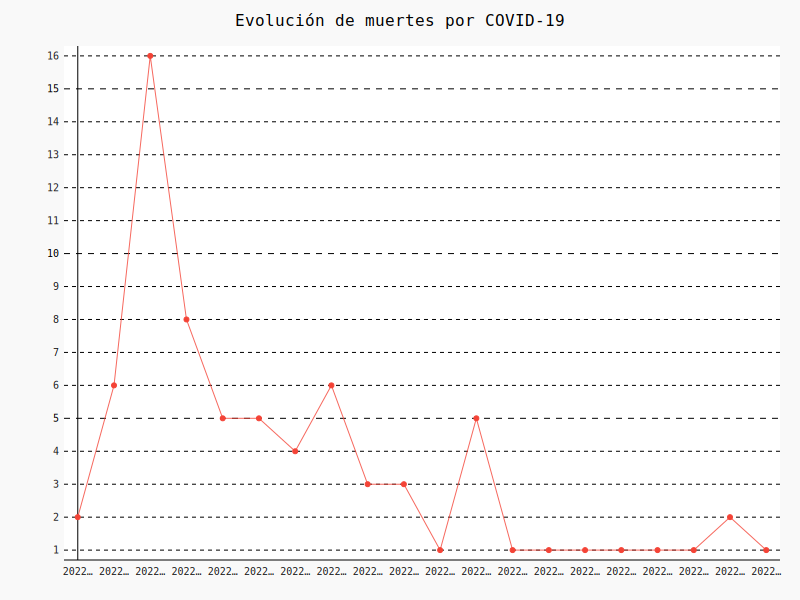
\includegraphics[width=\textwidth]{pygal_linea}
		\caption{Implementación en Pygal}
		\label{Fig: PygalLinea}
	\end{subfigure}
	\caption{Implementación de gráfico de línea en diversos paquetes de visualización de datos.}
	\label{Fig: Linea}
\end{figure}

\subsubsection{Gráfico de barras}
La Figra \ref{Fig: Barras} muestra el resultado de la implementación de un gráfico de barras en los paquetes de visualización de datos \emph{Bokeh} (Figura \ref{Fig: BokehBarras}) y \emph{Pygal} (Figura \ref{Fig: PygalBarras}).

\begin{figure}[!htb]
	\centering
	\begin{subfigure}[b]{0.4\textwidth}
		\centering
		\includegraphics[width=\textwidth]{bokeh_barras}
		\caption{Implementación en Bokeh}
		\label{Fig: BokehBarras}
	\end{subfigure}
	\begin{subfigure}[b]{0.4\textwidth}
		\centering
		\includegraphics[width=\textwidth]{pygal_barras}
		\caption{Implementación en Pygal}
		\label{Fig: PygalBarras}
	\end{subfigure}
	\caption{Implementación de gráfico de barras en diversos paquetes de visualización de datos.}
	\label{Fig: Barras}
\end{figure}

\newpage

\subsubsection{Histograma}
La Figra \ref{Fig: Histograma} muestra el resultado de la implementación de un histograma en los paquetes de visualización de datos \emph{Bokeh} (Figura \ref{Fig: BokehHistograma}) y \emph{Pygal} (Figura \ref{Fig: PygalHistograma}).

\begin{figure}[!htb]
	\centering
	\begin{subfigure}[b]{0.4\textwidth}
		\centering
		\includegraphics[width=\textwidth]{bokeh_histograma}
		\caption{Implementación en Bokeh}
		\label{Fig: BokehHistograma}
	\end{subfigure}
	\begin{subfigure}[b]{0.4\textwidth}
		\centering
		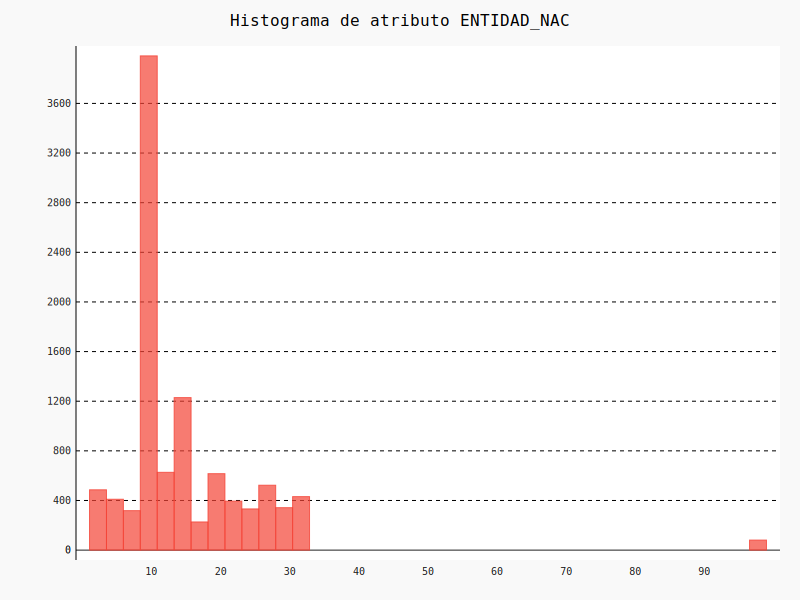
\includegraphics[width=\textwidth]{pygal_histograma}
		\caption{Implementación en Pygal}
		\label{Fig: PygalHistograma}
	\end{subfigure}
	\caption{Implementación de histograma en diversos paquetes de visualización de datos.}
	\label{Fig: Histograma}
\end{figure}

\subsubsection{Gráfico de dispersión}
La Figra \ref{Fig: Dispersion} muestra el resultado de la implementación de un gráfico de dispersión en los paquetes de visualización de datos \emph{Bokeh} (Figura \ref{Fig: BokehDispersion}) y \emph{Pygal} (Figura \ref{Fig: PygalDispersion}).

\begin{figure}[!htb]
	\centering
	\begin{subfigure}[b]{0.4\textwidth}
		\centering
		\includegraphics[width=\textwidth]{bokeh_dispersion}
		\caption{Implementación en Bokeh}
		\label{Fig: BokehDispersion}
	\end{subfigure}
	\begin{subfigure}[b]{0.4\textwidth}
		\centering
		\includegraphics[width=\textwidth]{pygal_dispersion}
		\caption{Implementación en Pygal}
		\label{Fig: PygalDispersion}
	\end{subfigure}
	\caption{Implementación de gráfico de dispersión en diversos paquetes de visualización de datos.}
	\label{Fig: Dispersion}
\end{figure}

\subsubsection{Gráfico de pastel}
La Figra \ref{Fig: Pastel} muestra el resultado de la implementación de un gráfico de pastel en los paquetes de visualización de datos \emph{Bokeh} (Figura \ref{Fig: BokehPastel}) y \emph{Pygal} (Figura \ref{Fig: PygalPastel}).

\begin{figure}[!htb]
	\centering
	\begin{subfigure}[b]{0.4\textwidth}
		\centering
		\includegraphics[width=\textwidth]{bokeh_pastel}
		\caption{Implementación en Bokeh}
		\label{Fig: BokehPastel}
	\end{subfigure}
	\begin{subfigure}[b]{0.4\textwidth}
		\centering
		\includegraphics[width=\textwidth]{pygal_pastel}
		\caption{Implementación en Pygal}
		\label{Fig: PygalPastel}
	\end{subfigure}
	\caption{Implementación de gráfico de pastel en diversos paquetes de visualización de datos.}
	\label{Fig: Pastel}
\end{figure}

\newpage

\subsubsection{Diagrama de cajas}
La Figra \ref{Fig: Cajas} muestra el resultado de la implementación de un diagrama de cajas en los paquetes de visualización de datos \emph{Bokeh} (Figura \ref{Fig: BokehCajas}) y \emph{Pygal} (Figura \ref{Fig: PygalCajas}).

\begin{figure}[!htb]
	\centering
	\begin{subfigure}[b]{0.4\textwidth}
		\centering
		\includegraphics[width=\textwidth]{bokeh_cajas}
		\caption{Implementación en Bokeh}
		\label{Fig: BokehCajas}
	\end{subfigure}
	\begin{subfigure}[b]{0.4\textwidth}
		\centering
		\includegraphics[width=\textwidth]{pygal_cajas}
		\caption{Implementación en Pygal}
		\label{Fig: PygalCajas}
	\end{subfigure}
	\caption{Implementación de diagrama de cajas en diversos paquetes de visualización de datos.}
	\label{Fig: Cajas}
\end{figure}



\section{Conclusiones}
El manejo de datos faltantes siempre presenta un gran reto dentro del área de inteligencia artificial. Los métodos analizados e implementados en esta práctica han demostrado ser útiles para llenar estos espacios vacíos y no cambiar la distribución original de los datos.

Hablando específicamente de cada uno de los atributos trabajados tenemos:

\begin{itemize}
	\item \textbf{sex}. Dado a que solamente había 3 datos faltantes, fue bastante claro el implementar un método como la imputación por moda. Habría que investigar si dicho método es recomendable solamente ante ciertos rangos de datos faltantes.
	
	\item \textbf{hypertension}. Considerando que el índice de correlación máximo obtenido coincide con la variable objetivo, fue fácil imaginar que la imputación por media/moda de clases sería ideal, sin embargo al prestar atención al método podemos observar que la distribución de los posibles valores de este atributo es aproximadamente de 3:1, por lo que el método de moda de clase rellenó todos los faltantes con la clase 0, mismo resultado se hubiera obtenido con una imputación por moda y hubiera disminuido la complejidad computacional.
	
	\item \textbf{workt\_type y Residence\_type}. El método de imputación aleatoria logró mantener de forma adecuada la distribución de estas variables, comportamiento que se atribuye a la claras diferencias en la frecuencia de cada una de las observaciones de cada atributo, es muy probable que utilizar este método en atributos con mayor resolución no será eficaz.
	
	\item \textbf{bmi}. Considerar que el mayor índice de correlación fue con el atributo \emph{avg\_glucose\_level} fue de ayuda para lograr estimar una línea de tendencia entre ambos atributos, sin embargo, dicho valor de correlación apenas fue de $0.24$, lo cuál es un claro indicador de que no existe una relación lineal entre ambos atributos (afirmación que se confirma al generar un gráfico de dispersión entre ambos atributos (Figura \ref{Fig: Dispersion})). Existe la posibilidad de que utilizar algún tipo de regresión no lineal pueda mejorar el rendimiento de este método. A pesar de sus limitantes, es destacable el hecho de que se logró conservar la forma de la distribución de los datos originales.
\end{itemize}

\begin{figure}[htbp]
	\centering
	\includegraphics[width=0.8\textwidth]{bmi_glucose}
\end{figure}


% \nocite{*}
\renewcommand{\refname}{Referencias bibliográficas}
\bibliographystyle{IEEEtran-spanish}
\bibliography{referencias}

\appendix
\section{Código documentado}
El código completo y funcional se puede encontrar anexo en el archivo \emph{zip} compartido en conjunto con este reporte, así como en las secciones anexas.

\subsection{DeleteData.py}
Script implementado para generar datos faltantes.
\lstinputlisting[language=Python]{../DeleteData.py}

\subsection{Practica2\_EnriqueMenaCamilo.py}
Script implementado para el desarrollo de la práctica.
\lstinputlisting[language=Python]{../Practica2_EnriqueMenaCamilo.py}

\end{document}